\documentclass{llncs}[11pt]

\def\isanonymous{0}
\def\isshort{0}

\usepackage{ifthen}
\newcommand{\anonymous}[2]{
\ifthenelse{\equal{\isanonymous}{1}}
{{#1}}
{{#2}}
}

\newcommand{\submission}[2]{\ifthenelse{\equal{\isshort}{1}}{{#1}\xspace}{{#2}\xspace}}


\ifthenelse{\equal{\isshort}{0}}{
\usepackage{a4wide}
}{}

\usepackage[utf8x]{inputenc}
\usepackage{amsmath,amsfonts,amssymb}
\usepackage{xspace}
\usepackage{tikz,pgfplots}

%%%%%%%%%%%%%%%%%%%%%%%%%%%%%%%%%%%%%%%%%%%%%%%%%%%%%%%%%%%%%%%%
% Speed up compilation by caching Tikz picktures
%
% when you change a tikz picture run: 
%
%  pdflatex -shell-escape bkw-small-secret
%
% You can also simply comment out the two lines below to go back 
% to the normal behaviour
%%%%%%%%%%%%%%%%%%%%%%%%%%%%%%%%%%%%%%%%%%%%%%%%%%%%%%%%%%%%%%%%

%\usetikzlibrary{external}
%\tikzexternalize[prefix=figures/] % activate!

\usepackage{embedfile}

\usepackage{url}
\usepackage[vlined,linesnumbered]{algorithm2e}

\usepackage[index,multiuser]{fixme}
\fxsetup{
    status=draft,
    layout=pdfcnote,
    theme=color
}

\FXRegisterAuthor{malb}{amalb}{malb}
\FXRegisterAuthor{lp}{alp}{lp}
\FXRegisterAuthor{rf}{arf}{rf}

\newcommand\LWE{\ensuremath{{\rm LWE}}\xspace}
\newtheorem{assumption}{Assumption}

\newcommand{\tildeO}[1]{\ensuremath{\tilde{\mathcal{O}}(#1)}\xspace}

\newcommand{\heading}[1]{{\vspace{6pt}\noindent\sc{#1.}}}

\newcommand{\bigO}[1]{\ensuremath{\mathcal{O}\left(#1\right)}\xspace}
\newcommand{\poly}{ {\rm poly}(n)}
\newcommand{\chig}{\ensuremath{\chi_{\alpha,q}}}
\newcommand{\chis}{\ensuremath{\psi}}
\newcommand{\U}[1]{\ensuremath{\mathcal{U}(#1)\xspace}}
\newcommand{\Z}{\ensuremath{\mathbb{Z}}\xspace}
\newcommand{\Zq}{\ensuremath{\mathbb{Z}_q}\xspace}
\newcommand{\Zp}{\ensuremath{\mathbb{Z}_p}\xspace}
\newcommand{\Zqchi}{\ensuremath{\mathbb{Z}^{\Phi_{\zeta}}_q}[\vec{x}]\xspace}
\newcommand{\Ldis}{L_{\mathbf{s},\chi}\xspace}

\newcommand{\Bdis}[1]{B_{\mathbf{s},\chi}(b,#1,p)\xspace}
\newcommand{\Bdissm}[1]{B_{small,\mathbf{s},\chi}(b,#1,p)\xspace}
\newcommand{\sample}{\ensuremath{\leftarrow_{\$}}}

\newcommand{\CDF}[1]{\textnormal{CDF}\left(#1\right)\xspace}
\newcommand{\E}{\ensuremath{\textnormal{E}}}
\newcommand{\Var}{\ensuremath{\textnormal{Var}}}

\newcommand{\abs}[1]{\ensuremath{\left|#1\right|}\xspace}

\renewcommand{\vec}[1]{\mathbf{#1}\xspace}
\newcommand{\shortvec}[1]{\tilde{\mathbf{#1}}\xspace}
\newcommand{\mat}[1]{\ensuremath{\mathbf{#1}}\xspace}

\newcommand{\dotp}[2]{\ensuremath{\left\langle {#1},{#2}\right\rangle}\xspace}
\newcommand{\N}[1]{\ensuremath{\mathcal{N}({#1)}}}
\newcommand{\round}[1]{\ensuremath{\left\lfloor{#1}\right\rceil}\xspace}

\def\abn{\lceil n/b \rceil}


\title{Lazy Modulus Switching for the BKW Algorithm on LWE}
\anonymous{\author{} \institute{}}{
\author{Martin R.~Albrecht \inst{1} \and Jean-Charles Faugère \inst{3,2,4} \and Robert Fitzpatrick \inst{5} \and Ludovic Perret \inst{2,3,4}}
\institute{
Technical University of Denmark, Denmark \and
Sorbonne Universités, UPMC Univ Paris 06, POLSYS, UMR 7606, LIP6, F-75005, Paris, France \and
INRIA, Paris-Rocquencourt Center, POLSYS Project\and
CNRS, UMR 7606, LIP6, F-75005, Paris, France \and
Information Security Group\\
Royal Holloway, University of London\\
Egham, Surrey TW20 0EX, United Kingdom \\ 
\email{maroa@dtu.dk, jean-charles.faugere@inria.fr, robert.fitzpatrick.2010@live.rhul.ac.uk, ludovic.perret@lip6.fr}  
}}


\parindent 0em
\parskip 0.9em

\begin{document}

\maketitle

\begin{abstract}
Some recent constructions based on LWE do not sample the secret uniformly at random but rather from some distribution which produces small entries. The most prominent of these is the binary-LWE problem where the secret vector is sampled from $\{0,1\}^{\ast}$ or $\{-1,0,1\}^{\ast}$. We present a variant of the BKW algorithm for binary-LWE and other small secret variants and show that this variant reduces the complexity for solving binary-LWE. We also give estimates for the cost of solving binary-LWE instances in this setting and demonstrate the advantage of this BKW variant over  standard BKW and lattice reduction techniques applied to the SIS problem. Our variant can be seen as a combination of the BKW algorithm with a lazy variant of modulus switching which might be of independent interest.
\end{abstract}

\section{Introduction} \label{sec:intro}
Learning With Errors (\LWE) \cite{regev:acm09} has received  widespread attention from the cryptographic community since its introduction. \LWE-based cryptography is mainly motivated by its great flexibility for instantiating cryptographic solution as well as a deep worst-case/average-case connections \cite{regev:acm09}: solving \LWE{} on the average is not easier than solving worst-case instances of several famous lattice approximation problems.

The motivation behind this work comes from the observation that some recent constructions based on \LWE do not sample the secret uniformly at random but rather from some distribution which produces small entries (e.g.\ \cite{applebaum-cash-peikert-sahai:crypto2009,DBLP:conf/tcc/AkaviaGV09,DBLP:conf/innovations/GoldwasserKPV10,gentry-halevi-smart:crypto2012,DBLP:conf/tcc/Pietrzak12}). From a theoretical point of view, this is motivated by the observation that every \LWE instance can be transformed into an instance where the secret follows the same distribution as the noise \cite{applebaum-cash-peikert-sahai:crypto2009}.\footnote{also in \cite{kirchner:eprint2011} for the LPN case.} However, many constructions use secrets which are considerably smaller.
For example, binary-\LWE samples the secret from $\{0,1\}^*$ \cite{brakerski-langlois-peikert-regev-stehle:stoc13} or $\{-1,0,1\}^*$ \cite{gentry-halevi-smart:crypto2012}. The presence of such small secrets provokes the question of what implications such choices have on the security of \LWE. Is solving \LWE with, say, binary secrets easier than standard \LWE? From a theoretical point of view, \cite{brakerski-langlois-peikert-regev-stehle:stoc13} proves that their binary-\LWE is as secure as \LWE{}. In this paper, we try to address the question from an algorithmic point of view; i.e. what is the actual impact of small secrets on concrete parameters.    

\subsection{Algorithms for Solving \LWE}
Three families of algorithms for solving \LWE are known in the literature. The most prominent approach is to reduce \LWE to a problem that can be solved via lattice reduction, for example, by reducing it to the Short Integer Solution (SIS) problem. Indeed, most parameter choices in the literature are based on the hardness of lattice reduction such as \cite{LindnerP10,chen-nguyen:asiacrypt2011,liu-nguyen:ctrsa2013}. These estimates for a given set of parameters $n$ (number of components of the secret), $q$ (size of the modulus) and  $\sigma$ (standard deviation of the noise) are usually produced by extrapolating running times from small instances.

A second approach is due to Arora and Ge who reduce \LWE to solving a  system of non-linear equations \cite{arora-ge:icalp2011}. This algorithm allow us to solve \LWE in sub-exponential time as soon as the Gaussian distribution  is sufficiently narrow, i.e.\ $\alpha \cdot q <\sqrt{n}$. Recall that  the security reduction \cite{regev:acm09} for \LWE requires to consider discrete Gaussian  with standard deviation $\alpha \cdot q$ strictly bigger than $\sqrt{n}$.
However, from a practical point of view, the constants involved in this algorithm are so large that it is much more costly than other approaches for the parameters typically considered in cryptographic applications \cite{SCC12_AG}. 

The third family of algorithms are combinatorial algorithms which can all be seen as variants of the BKW algorithm. The BKW algorithm was proposed by Blum, Kalai and Wasserman~\cite{blum-kalai-wasserman:acm2003} as a method for solving the Learning Parity with Noise problem, with sub-exponential complexity, requiring $2^{\bigO{n / \log n}}$ samples, space and time. The algorithm can be adapted for tackling \LWE with complexity $2^{\bigO{n}}$ when the modulus is taken to be polynomial in $n$ \cite{regev:acm09}. BKW proceeds by splitting the $n$ components of LWE samples into $a$ groups of $b$ components each. For each of the $a$ groups of components the algorithm then searches for collisions in these $b$ components to eliminate them. The overall complexity of the algorithm is  $\approx \left(a^2n\right) \cdot \frac{q^b}{2}$ operations, and $a\cdot \frac{q^b}{2}$ memory, where $a$ and $b$ depend on the $n, q$ and $\alpha$.

The behaviour of the algorithm is relatively well understood and it was shown to outperform lattice reduction estimates when reducing LWE to SIS (when $q$ is small), thus it provides a solid basis for analysing the concrete hardness of LWE instances \cite{albrecht-cid-faugere-fitzpatrick-perret:dcc2013}.

\subsection{Organisation of the Paper and Main Results}
While none of the algorithms above take advantage of the presence of small secrets, we may combine them with  {\it modulus switching}. Recall that modulus switching was initially introduced to improve the performance of homomorphic encryption schemes \cite{brakerski-vaikuntanathan:focs2011} and was recently used to reduce the hardness of \LWE with polynomially sized moduli to GAPSVP \cite{brakerski-langlois-peikert-regev-stehle:stoc13}. Modulus switching is essentially the same as computing with a lower precision similar to performing floating point computations with a low fixed precision. Namely, let $\big(\vec{a},
c=\dotp{\vec{a}}{\vec{s}} + e\big) \in \Zq^n \times \Zq$ be \LWE sample 
where $\vec{s} \in \Zq^n$ is the secret vector, and $e \in \Zq$ is an error. Let also some $p < q $ and consider $\big(\round{{p}/{q} \cdot \vec{a}}, \round{{p}/{q} \cdot c}\big)$ with
\begin{small}
\begin{align}
\label{eq:roundingerror}
\round{\frac{p}{q} \cdot c} =& \round{\frac{p}{q} \big( \dotp{\vec{a}}{\vec{s}}+q \cdot u +e \big)}, \mbox{ for some $u \in \Z$}\nonumber\\
\round{\frac{p}{q} \cdot c} =& \round{ \dotp{ \frac{p}{q} \cdot \vec{a} }{\vec{s} }_{p} + \frac{p}{q} \cdot e} =  \round{ \dotp{ \round{ \frac{p}{q} \cdot \vec{a} }}{\vec{s} }_{p} + \dotp{\frac{p}{q} \cdot \vec{a} - \round{ \frac{p}{q} \cdot \vec{a} }}{\vec{s}}_{p} + \frac{p}{q} \cdot e}\nonumber\\
  =& \dotp{ \round{ \frac{p}{q} \cdot \vec{a} }}{\vec{s} }_{p} + \dotp{\frac{p}{q} \cdot \vec{a} - \round{ \frac{p}{q} \cdot \vec{a} }}{\vec{s}}_{p} + \frac{p}{q} \cdot e + e' \textnormal{, where } e' \in [-0.5,0.5] \nonumber\\
  =& \dotp{ \round{ \frac{p}{q} \cdot \vec{a} }}{\vec{s} }_{p} + e'' + \frac{p}{q}\cdot e + e'.
\end{align}
\end{small}
where $\dotp{\vec{x}}{\vec{y}}_{p}$ denotes the modulo $p$ inner product of $\vec{x}$ and $\vec{y}$.

Since ${p}/{q} \cdot \vec{a} - \round{ {p}/{q} \cdot \vec{a} }$ takes values $\in [-0.5,0.5]$ we have that $e''$ is small if $\vec{s}$ is small. We may hence compute with the smaller `precision' $p$ 
at the cost of a slight increase of the noise rate by  a `{\it rounding error}' $e''$. 
 
Modulus switching allows to map a \LWE{} instance $\bmod \, q$ to a scaled instance of \LWE{} $\bmod \, p$.
Thus, modulus switching can be used in the solving of small secret instances of \LWE, a folklore approach which has not been explicitly studied in the literature. Namely, if we pick $p$ such that $e''$ is not much larger than $p/q \cdot e$ then, for example, the running time of the BKW 
algorithm improves from $(a^2n)\cdot \frac{q^b}{2}$ to $(a^2n)\cdot \frac{p^b}{2}$. Since typically $b \approx n/\log n$ 
this may translate to substantial improvements. Indeed, we can pick $p$ such that $\abs{\dotp{{p}/{q} \cdot \vec{a} - 
\round{ {p}/{q} \cdot \vec{a} }}{\vec{s}}} \approx p/q \cdot \abs{e}$.
This implies ${\sigma_s}\cdot \sqrt{\frac{n}{12}} \approx p/q \cdot \sigma$, or
$
p \approx \min\left\{q, \frac{\sigma_s}{\sigma}\cdot \sqrt{\frac{n}{12}} \cdot q \right\}$, where $\sigma_s$ is the standard deviation of elements in the secret $\vec{s}$.

In this paper, we refine this approach and present a variant of the BKW algorithm which fuses modulus switching and BKW-style reduction. In particular, this work has two main contributions. Firstly, in Section~\ref{sec:bkw-algorithm} we present a modulus switching strategy for the BKW algorithm in which switching is delayed until necessary.  In a nutshell, recall that the BKW algorithm performs additions of elements which collide in certain components. Our variant will search for such collisions in `low precision' $\Zp$ but will perform arithmetic in `high precision' $\Zq$.  We call {\it rounding error} the inner product of the sub-vector of `low bits' of $\vec{a}$ with the secret $\vec{s}$. Our strategy permits to decrease rounding errors and allows to reduce $p$ by a factor of $\sqrt{a}$.

Secondly, this perspective enables us to choose reductors in the BKW algorithm which minimise the rounding errors further (Section \ref{sec:control-growth}). Namely, we favour components $a$ with small distance $\abs{\round{ {p}/{q} \cdot a} - {p}/{q} \cdot a}$ in already reduced components, called `child components' in this work. Our strategy ensures that the probability of finding such elements is highest for those components which are considered first by the BKW algorithm, i.e.\ those components which contribute most to the noise. We note that the first contribution relies on standard independence assumptions only, while the second contribution relies on stronger assumptions, which however seem to hold  in practice.

\def\polyfactor{n\, \log_2^2 n}
We then discuss the complexity of our variants in Section~\ref{sec:complexity}. For typical choices of parameters --  i.e.\ $q \approx n^c$ for some small constant $c\geq 1$, $a = \log_2 n$ and $b = n/\log_2 n$ --  the complexity of BKW  as analysed in \cite{albrecht-cid-faugere-fitzpatrick-perret:dcc2013} 
is $\bigO{2^{cn}\cdot \polyfactor}$. For small secrets, a naive modulus switching technique allows reducing this complexity to  
$\bigO{2^{n\big(c+\frac{\log_2 d}{\log_2 n}\big)} \cdot \polyfactor}$ where $0<d\leq 1$ is a small constant. 
\begin{comment}
sage: n,c,d = var('n,c,d')
sage: assume(c>0)
sage: assume(c, 'integer')
sage: assume(n>0)
sage: assume(d<=1)
sage: assume(d>0)
sage: q = n^c
sage: b = n/log(n)
sage: a = log(n)
sage: sigma = sqrt(n)
sage: p = d*q/sqrt(a)
sage: f = e^(n*log(d)/log(n)) # d^(n/log(n)), base e
sage: g = e^(c*n) # n^(c*n/log(n)) 
sage: h = (1/sqrt(log(n)))^(n/log(n))
sage: assert( bool(f*g*h == p^b) == True ) 
sage: simple = e^(n*(c+ (log(d)-1/2*log(log(n)))/log(n)))
sage: assert( bool(simple == p^b) == True ) 
\end{comment}
If the secret distribution does not depend on $n$ and if an unbounded number of \LWE samples is available our improved version of BKW allows to get a complexity of:
\def\complexity{\bigO{2^{n\big(c+\frac{\log_2 d-\frac 1 2 \log_2 \log_2 n}{\log_2 n}\big)}\cdot \polyfactor}}
$$ 
\complexity.
$$
We then study the behaviour of this algorithm by applying it to various instances of LWE with binary secrets. \submission{}{In Section~\ref{sec:implementation} we report on experiments conducted with a proof-of-concept implementation of our algorithm.} In Section~\ref{sec:parameters},
we compare the results with plain BKW and BKZ under modulus switching and a simple meet-in-the-middle approach or generalised birthday attack. We show that our lazy-modulus-switching variant of the BKW algorithm provides better results than applying plain BKW after modulus reduction. We also demonstrate that under the parameters considered here this algorithm also -- as $n$ increases -- outperforms the most optimistic estimates for BKZ when we apply BKZ to the same task as that to which we apply BKW: finding short vectors in the (scaled-)dual lattice -- we obtain this perspective by viewing the rounding error as an increase in the noise rate while still finding short vectors in the \mbox{(scaled)-}dual $p$-ary lattice determined by our modulus-reduced LWE samples. Indeed, our results indicate that our algorithm outperforms BKZ 2.0 when both are used to find a short vector in the \mbox{(scaled)-}dual lattice in dimension as low as $\approx 256$ when considering \LWE{} parameters from \cite{regev:acm09} with binary secret. However, we stress again that we always assume an unbounded number of samples to be available for solving.

\subsection{Notations}
To fix the notations, we reproduce below the definition of \LWE{}.
\begin{definition}[LWE \cite{regev:acm09}]\label{def:lwe} Let $n,\, q$ be positive integers, $\chi$ be a probability distribution on $\Zq$ and $\vec{s}$ be a secret vector in $\Zq^n$. We denote by $\Ldis$ the probability distribution on $\Zq^n \times \Zq$ obtained by choosing $\vec{a}\in \Zq^n$ uniformly at random, choosing $e \in \Zq$ according to $\chi$, and returning  $(\vec{a},c)=(\vec{a},\dotp{\vec{a}}{\vec{s}}+ e) \in \Zq^n \times \Zq.$ We define 
\textnormal{Decision-LWE} as the problem of deciding whether pairs $(\vec{a},c)\in \Zq^n \times \Zq$ are sampled according to $\Ldis$ or the uniform distribution on $\Zq^n \times \Zq$. \textnormal{Search-LWE} is the problem of recovering $\vec{s}$ from $(\vec{a},c)=(\vec{a},\dotp{\vec{a}}{\vec{s}}+ e) \in \Zq^n \times \Zq$ sampled according to $\Ldis$.  
\end{definition}
The noise follows some distribution $\chi$ which is classically chosen to be a discrete Gaussian distribution over $\Z$ with mean $0$ and standard deviation $\sigma = s/\sqrt{2 \pi} = \alpha q /\sqrt{2\pi}$, reduced modulo $q$.
In the following, we always start counting at zero.  We denote vectors as well as  matrices in bold, vectors in lower case, and matrices in upper case. Given a vector $\vec{a}$, we denote by $\vec{a}_{(i)}$ the $i$-th entry in $\vec{a}$, i.e.\ a scalar, and by $\mat{A}_{(i,j)}$ the entry at index $i,j$. For vectors $\vec{a}$ we denote by $\vec{a}_{(a,b)}$ the vector $(\vec{a}_{(a)},\dots,\vec{a}_{(b-1}))$. 
When given a list of vectors, we index its elements by subscript, e.g.\ $\vec{a}_0,\vec{a}_1, \vec{a}_2$, to denote the first 
three vectors of the list. This means that $\vec{a}_{i,(j)}$ is the $j$-th component of the vector $\vec{a}_i$.  When we write $(\vec{a}_i,c_i)$ we always mean the output of an oracle which should be clear from the context. In particular, $(\vec{a}_i,c_i)$ does not necessarily refer to samples following the initial distribution. We write $\shortvec{a}$ instead of $\vec{a}$ to indicate $\vec{a}$ has some short elements. 
We represent elements in $\Zq$ as integers in $[-\frac{q}{2},\ldots,\frac{q}{2}]$, similarly for $\Zp$. We write $\chig$ for the distribution obtained by considering a discrete Gaussian distribution over $\Z$ with standard deviation $\alpha q /\sqrt{2\pi}$, mean $0$, considered modulo $q$.

\section{The BKW Algorithm}
\label{sec:bkw-algorithm}

The BKW algorithm was proposed by Blum, Kalai and Wasserman~\cite{DBLP:journals/jacm/BlumKW03} as a method for solving the LPN problem, with sub-exponential complexity, requiring $2^{\bigO{n / \log n}}$ samples and time. The algorithm can be adapted for tackling Search- and Decision-LWE, with complexity $2^{\bigO{n}}$, when the modulus is taken to be polynomial in $n$. 

To describe and analyse the BKW algorithm we use terminology and intuitions from linear algebra. Recall that noise-free linear systems of equations are solved by (a) transforming them into a triangular shape, (b) recovering a candidate solution in one variable for the univariate linear equation produced and (c) extending this solution by back substitution. Similarly, if we are only interested in \emph{deciding} whether a linear system of equations does have a common solution, the standard technique is to produce a triangular basis and express other rows as linear combinations of this basis, i.e., to attempt to reduce them to zero.

The BKW algorithm -- when applied to Search-LWE -- can be viewed as consisting of three stages somewhat analogous to those of linear system solving: 
\begin{description}
 \item[(a) sample reduction] is a form of Gaussian elimination which, instead of treating each component independently, considers `blocks' of $b$ components per iteration, where $b$ is a parameter of the algorithm.
 \item[(b) hypothesis testing] tests candidate sub-solutions to recover components of the secret vector {\bf s}.
 \item[(c) back substitution] such that the whole process can be continued on a smaller LWE instance.
\end{description}

On a high-level, to aid intuition, if the standard deviation of $\chi$ was zero and hence all equations were noise-free, we could obviously recover $\svec$ by simple Gaussian elimination. When we have non-zero noise, however, the number of row-additions conducted during Gaussian elimination result in the noise being `amplified' to such levels that recovery of $\svec$ would generally be impossible. Thus the motivation behind the BKW algorithm can be thought of as using a greater number of rows but eliminating many variables with single additions of rows rather than just one. If we can perform a Gaussian elimination-like reduction of the sample matrix using few enough row additions, the resulting noise in the system is still `low enough' to allow us to recover one or a few components of $\svec$ at a time. While, mainly for convenience of analysis, we choose a nested-oracle approach below to define the algorithm, the above intuitive approach is essentially equivalent.

The way we study the complexity of the BKW algorithm for solving the LWE problem is closely related to the method described in~\cite{FL06}: given an oracle that returns samples according to the probability distribution $\Ldis$, we use the algorithm's first stage to construct an oracle returning samples according to another distribution, which we call $\Bdis{a}$, where $a = \abn$ denotes the number of `levels' of addition. The complexity of the algorithm is related to the number of operations performed in this transformation, to obtain the required number of samples for hypothesis testing.

We now study the complexity of the first stage of the BKW algorithm.

\subsection{Sample Reduction}

Given $n \in \Z$, select a positive integer $b\leq n$ (the window width), and let $a:= \abn$ (the addition depth).
Given an LWE oracle (which by abuse of notation, we will also denote by $\Ldis$), we denote by ${\Bdis{\ell}}$ a related oracle which outputs samples where the first $b \cdot \ell$ coordinates of each $\avec_i$ are zero, generated under the distribution (which again by abuse of notation, we denote by ${\Bdis{\ell}}$) obtained as follows: 
\begin{itemize}
\item if $\ell=0$, then $\Bdis{0}$ is simply $\Ldis$;
\item if $0<\ell<a$, the distribution $\Bdis{\ell}$ is obtained by taking the difference of two vectors from $\Bdis{\ell-1}$ that agree on the elements 
$(\avec_{((\ell-1)\cdot b)},\avec_{((\ell-1)\cdot b+1)},\ldots,\avec_{(\ell\cdot b-1)}).$
\end{itemize}
We can then describe the first stage of the BKW algorithm as the (recursively constructed) series of sample oracles ${\Bdis{\ell}}$, for $0 \leq \ell <  a$. Indeed, we define ${\Bdis{0}}$ as the oracle which simply returns samples from $\Ldis$, while ${\Bdis{\ell}}$ is constructed from ${\Bdis{\ell-1}}$, for $\ell \geq 1$. We will make use of a set of tables $T$ (maintained across oracle calls) to store (randomly-chosen) vectors that will be used to reduce samples arising from our oracles. 
More explicitly, given a parameter $b \leq n$ for the window width, and letting $a = \abn$, we can describe the oracle ${\Bdis{\ell}}$ as  follows:
\begin{enumerate}
\item For $\ell = 0$, we can obtain samples from ${\Bdis{0}}$ by simply calling the LWE oracle $\Ldis$ and returning the output.
\item For $\ell = 1$, we repeatedly query the oracle ${\Bdis{0}}$ to obtain (at most) $(q^b-1)/2$ samples $(\avec,c)$ with distinct non-zero vectors for the first $b$ coordinates of $\avec$. We only collect $(q^b-1)/2$ such vectors because we exploit the symmetry of $\Zq$ and that of the noise distribution. We use these samples to populate the table $T^1$, indexed by the first $b$ entries of $\avec$. We store $(\avec, c)$ in the table. During this course of this population, whenever we obtain a sample $(\mathbf{a'},c')$ from ${\Bdis{0}}$, if either the first $b$ entries of $\mathbf{a}'$ (resp.\ their negation) match the first $b$ entries of a vector $\avec$ such that the pair $(\avec,c)$ is already in $T^1$, we return $(\avec'\pm \avec,c'\pm c)$, as a sample from ${\Bdis{1}}$. Note that, if the first $b$ entries in $\mathbf{a}'$ are zero, we return $(\mathbf{a}',c')$ as a sample from ${\Bdis{1}}$. Further calls to the oracle ${\Bdis{1}}$ proceed in a similar manner, but using (and potentially adding entries to) the same table $T^1$. 

\item For $1 < \ell < a$, we proceed as above:  we make use of the table $T^{\ell}$ (constructed by calling ${\Bdis{\ell - 1}}$ up to $(q^b-1)/2$ times) to reduce any output sample from ${\Bdis{\ell - 1}}$ which has the $b$ entries in its $\ell$-th block already in  $T^{\ell}$, to generate a sample from  ${\Bdis{\ell}}$.
\end{enumerate}

Pseudo-code for the oracle ${\Bdis{\ell}}$, for $0 < \ell < a$, is given in Algorithm~\ref{alg:bdis} (the case $\ell = a$ will be discussed below). 

\begin{algorithm}[H]
\label{alg:bdis}
\SetKw{KwAnd}{and}
\SetKw{KwOr}{or}
\KwIn{$b$ -- an integer $0 < b \leq n$}
\KwIn{$\ell$ -- an integer $0 < \ell < a$}
\Begin{
$T^{\ell} \gets$ array indexed by $\Zq^b$ maintained across all runs of ${\Bdis{\ell}}$\;
query ${\Bdis{\ell-1}}$ to obtain $(\avec,c)$\;
\If{$\avec_{(b\cdot(\ell-1),b\cdot\ell)}$ is all zero vector}{\Return $(\avec,c)$\;}
\While{$T^{\ell}_{\avec_{(b\cdot(\ell-1),b\cdot\ell})}  = \varnothing$ \KwAnd $T^{\ell}_{-\avec_{(b\cdot(\ell-1),b\cdot\ell})}  = \varnothing$}{
  $T^{\ell}_{\avec_{(b\cdot(\ell-1),b\cdot\ell)}} \gets (\avec,c)$\;
  query ${\Bdis{\ell-1}}$ to obtain $(\avec,c)$\;
  \If{$\avec_{(b\cdot(\ell-1),b\cdot\ell)}$ is all zero vector}{\Return $(\avec,c)$\;}
}
\eIf{$T^{\ell}_{\avec_{(b\cdot(\ell-1),b\cdot\ell})}  \neq \varnothing$}{
   $(\avec',c') \gets T^{\ell}_{\avec_{(b\cdot(\ell-1),b\cdot\ell)}}$\;
   \Return $(\avec - \avec',c - c')$\;
}{   $(\avec',c') \gets T^{\ell}_{-\avec_{(b\cdot(\ell-1),b\cdot\ell)}}$\;
   \Return $(\avec + \avec',c + c')$\;
}




}
\caption{${\Bdis{\ell}}$ for $0 < \ell < a$}
\end{algorithm}


Then, given an LWE oracle $\Ldis$ outputting samples of the form $(\avec,\dotp{\avec}{\svec} + e)$, where $\avec , \svec \in \Zq^n$, the oracle
${\Bdis{a-1}}$ can be seen as another LWE oracle outputting samples of the form $(\avec',\dotp{\avec'}{\solvec} + e')$, where $\avec' , \solvec \in \Zq^k$, with $k = n \bmod b$, if $b$ does not divide $n$, or $k=b$ otherwise,
and $e'$ is generated with a different distribution (related to the original error distribution and the value $a$).
The vector $\solvec$ is defined to be the last $k$ components of $\svec$. For the remainder of this section we will assume that $n \bmod b = 0$, and therefore $k=b$ (this is done to simplify the notation, but all the results obtained can be easily adapted when the last block has length $k < b$).

We note that, in our analysis below, we make the assumption for simplicity that all tables are completely filled during the elimination stage of the algorithm, thus giving conservative time and space bounds. In practise, especially in the final tables, this will not be the case and birthday-paradox arguments could be applied to derive a more realistic (lower) complexity. Typically,   if the number of samples required for hypothesis-testing is small, the birthday paradox implies that the storage required for the final table can be reduced by a square-root factor.

Moreover, in this work we introduce an additional parameter $d \leq b$ which does not exist in the original BKW algorithm~\cite{DBLP:journals/jacm/BlumKW03}. This parameter is used to reduce the number of hypotheses that need to be tested in the second stage of the algorithm, and arises from the fact we work with primes $q > 2$. At times, instead of working with the last block of length $b$, which could lead to potentially exponentially many hypotheses $q^b$ to be tested, 
we may employ a final reduction phase -- $\Bdis{a}$ -- to reduce the samples to $d<b$ non-zero entries in $\avec$. Thus $d$ will represent the number of components in our final block, i.e., the number of elements of the secret over which we conduct hypothesis tests. So after running the ${\Bdis{a-1}}$ algorithm, we may decide to split the final block to obtain vectors over $\Zq^d$. If so, we run the reduction function described above once more, which we will denote by $\Bdis{a}$. In the simple case where we do not split the last block (i.e., $d=b$), we adopt the convention that we will also call the $\Bdis{a}$ function, but it will perform no extra action (i.e., it simply calls ${\Bdis{a-1}}$). Thus we have that for a choice of $0 \leq d \leq b$, the oracle ${\Bdis{a}}$ will output samples of the form $(\avec',\dotp{\avec'}{\solvec} + e')$, where $\avec' , \solvec \in \Zq^d$. We pick $d=0$ in the decision variant.

\heading{On choosing $b$ and $d$} In general, as discussed above, choosing the parameter $d$ to be small (e.g. $1$ or $2$) leads to the best results. However, in general one could also relax the condition $d \leq b$ to $d \leq n$ where $d=n$ is equivalent to straight-forward exhaustive search. Finally, a natural question is -- should all the blocks be of equal length or should some be shorter than others? Intuitively, choosing blocks which are all of equal size (or as close as possible) appears to be the optimal strategy, though we do not formally investigate this here. To ease the presentation, we assume throughout this paper that this is  the case.

From the constructions above, it follows that the cost of one call to ${\Bdis{\ell}}$ is at most $\lceil q^b/2\rceil$ calls to ${\Bdis{\ell-1}}$. We also need at most one addition of two outputs of ${\Bdis{\ell-1}}$, which have the first $b\cdot \ell$ entries in common. This operation requires $n+1 -b\cdot \ell$ additions in $\Zq$. Furthermore, since we maintain $T^{\ell}$  across different runs of ${\Bdis{\ell}}$, this cost is amortised across different runs of ${\Bdis{\ell}}$. Hence, when $\ell > 0$ the cost of calling ${\Bdis{\ell}}$ a total of $m$ times  is upper bounded by:
$$m + \frac{q^b-1}{2} \mbox{ calls to } {\Bdis{\ell-1}} \mbox{ and } m \mbox{ additions of outputs of } {\Bdis{\ell-1}}.
$$
Overall we obtain Lemma~\ref{lem:firststep}.

\begin{lemma}
\label{lem:firststep}
Let $n\ge 1$ be the dimension of the LWE secret vector, $q$ be a positive integer, and $d,b \in \mathbb{Z}$ with $1 \le d \leq b \le n$, and define $a = \abn$. The cost of calling $\Bdis{a}$, which returns samples $(\avec_i,c_i)$ with at most the $d$ rightmost entries of $\avec_i$ non-zero, $m$ times is upper bounded by 
\begin{eqnarray*}
\naddssteponeexactT + \naddssteponeexactM \\< \naddssteponeT + \naddssteponeM
\end{eqnarray*}
additions in $\Zq$ and $\ncallsT + \ncallsM \mbox{ calls to } \Ldis.$
\end{lemma}

\begin{proof}
We may think of the $\Bdis{\ell}$ oracles as constructing the matrix 
\[
B = \left(\begin{array}{ccccccccccccc}
   T^1 &        &         &        &        &        & \\
 0     & \hdots &       0 &    T^2 &        &        &  \\
 0     & \hdots &       0 &      0 & \hdots & 0      &    T^3 &        &  \\
\vdots & \ddots &  \vdots & \vdots & \ddots & \vdots & \vdots & \ddots &  \\
 0     & \hdots &       0 &      0 & \hdots & 0      &      0 & \hdots & 0 & T^{a-1}\\
 0     & \hdots &       0 &      0 & \hdots & 0      &      0 & \hdots & 0 & 0 & T^{a}\\\
 0     & \hdots &       0 &      0 & \hdots & 0      &      0 & \hdots & 0 & \hdots & 0 & M\\
\end{array}\right)
\]
where, for $1 \leq i \leq a-1$, $T^i$ represents a submatrix of $(q^b-1)/2$ rows and 
$n+1 -b\cdot(i-1)$ columns (the $+1$ accounts for the $c_i$ column).
According to our convention, $T^a$ is either a submatrix of $(q^{b-d}-1)/2$ rows and 
$n+1 - b\cdot(a-1)$ columns if we split the last block (i.e. $d<b$), or an empty matrix.
Finally $M$ represents a submatrix with $m$ rows and $d + 1$ columns. 
The matrix $B$ has therefore at most $(a-1) \cdot ((q^b-1)/2) + ((q^{b-d}-1)/2) + m < \ncallsT + \ncallsM$ 
rows and hence needs as many calls to $\Ldis$ to be constructed. This proves the second 
claim.

For the upper-bound on the number of additions necessary in $\Zq$, we have the following (we treat the worst case, where full construction of all $T$ tables is necessary before obtaining any samples from $\Bdis{a}$): The construction of $a$ $T$-tables is required, only $a-1$ (at most) of which require additions.
\begin{enumerate}

\item The construction of table $T^1$ requires $0$ ring additions.

\item The construction of table $T^2$ requires at most $((q^{b}-1)/2)\cdot(n+1 - b)$ additions.

\item The construction of table $T^3$ requires at most $((q^{b}-1)/2)\cdot ((n+1 - b) + (n+1 - 2b) )$ additions.

\item In general, for $2<i < a$, the construction of table $T^i$ requires at most 
\begin{eqnarray*}
\left(\frac{q^b-1}{2}\right)\cdot \left( (i-1) \cdot (n+1) - \sum_{j=1}^{i-1}j\cdot b \right) 
& = & \left(\frac{q^b-1}{2}\right)\cdot(i-1)\cdot \left((n+1) - \frac{i}{2}\cdot b \right).
\end{eqnarray*}

\item The construction of $T^a$ - the above expression is an upper bound for $i=a$.

\item Thus, the construction of all the $T^i$ tables requires at most
\begin{equation*}
\left(\frac{q^b-1}{2}\right)\cdot   \sum_{j=2}^a \left((j-1) \cdot((n+1) -\frac{j}{2}\cdot b) \right) 
 =  \left(\frac{q^b-1}{2}\right)\cdot \left(  \frac{a(a-1)}{2}\cdot (n+1)  - \sum_{k=1}^{a-1} \frac{k(k+1)}{2}\cdot b \right)
\begin{comment}\\
& = & \left(\frac{q^b-1}{2}\right)\cdot \left(  \frac{a(a-1)}{2}\cdot (n+1)  - \frac{ba(a-1)}{4}-\frac{b}{2}\left(\sum_{k=1}^{a-1}{k^2}\right) \right)\\
\end{comment}
\end{equation*}
$$=\left(\frac{q^b-1}{2}\right)\cdot \left(  \frac{a(a-1)}{2}\cdot (n+1)  - \frac{ba(a-1)}{4}-\frac{b}{6}\left(
(a-1)^3+\frac{3}{2}(a-1)^2+\frac{1}{2}(a-1)\right) \right)$$
additions in $\Zq$.
\item Now, for the construction of our $m$ final samples, the construction of each of these 
samples requires at most
\begin{eqnarray*}
(n+1-b)+(n+ 1-2b)+\ldots+(n+1 -a\cdot b) & = & \sum_{i=1}^{a}{\left(n+1-ib\right)} \\
& < & a\cdot \left( (n+1) - \frac{n}{2} \right)\\
& = & \frac{a}{2}\cdot \left( n+2  \right)\\
\end{eqnarray*}
additions (in $\Zq$).

\item Thus, the number of additions (in $\Zq$) incurred through calling $\Bdis{a}$ $m$ times is upper-bounded by:
\begin{equation*}
\naddssteponeexactT + \naddssteponeexactM
\end{equation*}
\end{enumerate}
and this concludes the proof of the lemma.
\qed
\end{proof}

The memory requirements for storing the tables $T^i$ are established in Lemma~\ref{lem:firststepmemory} below.

\begin{lemma}
\label{lem:firststepmemory}
Let $n\ge 1$ be the dimension of the secret, $q$ be a positive integer, and $d,b \in \mathbb{Z}$ with $1 \le d \leq b \le n$, and define $a = \abn$. The memory required to store the table $T^i$ is upper bounded by 
\begin{equation*}
\nstore
\end{equation*}
$\Zq$ elements, each of which requires $\lceil\log_2(q)\rceil$ bits of storage.
\end{lemma}

\begin{proof}
The table $T^1$ has $\frac{q^b}{2}$ entries each of which holds $n+1$ elements of $\Zq$. The table $T^2$ has the same number of entries but holds on $n+1-b$ elements of $\Zq$. Overall, we get that all tables together hold
\begin{eqnarray*}
\sum_{i=1}^{a} \left( \frac{q^b}{2} \right) \cdot \bigg(n+1 - (i-1)b\bigg) &=& \left( \frac{q^b}{2} \right) \sum_{i=1}^{a} n+1 - (i-1)b\\
\begin{comment}
 &=& \left( \frac{q^b}{2} \right) \cdot \left( a(n+1+b) - b\frac{(a+1)a}{2}\right)\\
\end{comment}
 &=& \left( \frac{q^b}{2} \right) \cdot a\cdot \left(n+1 - b\frac{a-1}{2}\right)\\
\end{eqnarray*}
$\Zq$ elements.\qed
\end{proof}
Note however that, while the original LWE oracle $\Ldis$ may output zero vectors (which offer no information for the hypothesis tests in the search variant) with probability $q^{-n}$, the oracle $\Bdis{a}$ may output such zero vectors with noticeable probability. In particular, calling $\Bdis{a}$ $m$ times does not guarantee that we get $m$ samples with non-zero coefficients in $\avec_i$. The  probability of obtaining a zero vector from $\Bdis{a}$ is $\frac{1}{q^d}$, and thus expect to have to call the oracle $\Bdis{a}$ around ${q^d}/{(q^d-1)} \cdot m$ times to obtain $\approx m$ useful samples with good probability.




\subsection{Hypothesis Testing}
\label{sec:hypothesis}
To give concrete estimates for the time and data complexity of solving a Search-LWE instance using BKW, we formulate the problem of solving an LWE instance as the problem of distinguishing between two different distributions. Assume we have $m$ samples  in $\Zq^d \times \Zq$ from $\Bdis{a}$. It follows that we have $\Zq^d$ hypotheses to test. In what follows, we examine each hypothesis in turn and derive a hypothesised set of noise values as a result (each one corresponding to one of the $m$ samples). We show that if we have guessed incorrectly for the subvector $\solvec$ of $\svec$ then the distribution of these hypothesised noise elements will be (almost) uniform while if we guess correctly then these hypothesised noise elements will be distributed according to $\chi_{a}$.  That is, if we have that the noise distribution associated with samples from $\Ldis$ is $\chi = \chi_{\alpha,q}$, then it follows from  Lemmas~\ref{lem:noisedist} and \ref{lem:firststep} that the noise distribution of samples obtained from $\Bdis{\ell}$ follows 
$\chi_{\sqrt{2^{\ell}}\alpha,q}$ if all inputs are independent, i.e., we are adding $2^\ell$ discrete Gaussians and produce a discrete Gaussian with standard deviation increased by a factor of $\sqrt{2^\ell}$. For the sake of simplicity, we denote this distribution by $\chi_\ell$ in the remainder of this work and also assume that the oracle $\Bdis{a}$ performs non-trivial operations on the output of $\Bdis{a-1}$, i.e., the oracle $\Bdis{a}$ performs a further reduction step. In other words we assume that the final oracle $\Bdis{a}$ results in a further increase in the standard deviation of the noise distribution associated with the final samples which are used to test hypotheses for elements of $\svec$. We hence make the following assumption in this section:

\begin{assumption}
If we let $\solvec := \svec_{(n-d,n)} = (\svec_{(n-d)},\ldots,\svec_{(n-1)})$, then the output of ${\Bdis{a}}$  is generated as $$\avec \sample \Zq^d, e \sample \chi_{a}: (\avec,\dotp{\avec}{\solvec} + e).$$
\end{assumption}

\begin{remark}
This section only refers to the Search-LWE problem in which we assume $q$ is prime for ease of analysis and exposition. This restriction does not apply to our results below on the decision variant.
\end{remark}

For our hypothesis-testing strategies, we think of each of the samples returned by $\Bdis{a}$ as giving rise to many equations $$f_i =- c_i \pm j + \sum_{k=0}^{d-1} (\avec_i)_{(k)} x_{(k)}  \textnormal{ for } 0 \leq j < q/2.$$ Given a number of these samples, in order to get an estimate for $\solvec$, we run through $q^d$ hypotheses and compute an array of scores $S$ indexed by the possible guesses in $\Zq^d$. That is, a function $W$ assigns a weight to elements in $\Zq$ which represent the noise under the hypothesis $\svec' = \vvec$. For each guess $\vvec$ we sum over the weighted noises $W(-c_i + \sum_{k=0}^{d-1}(\avec_i)_{(k)}\cdot v_{(k)})$. If $W$ is such that the counter $S_\vvec$ grows proportionally to the likelihood that $\vvec$ is the correct guess, then the counter  $S_{\solvec}$ will grow fastest. Pseudo-code is given in Algorithm~\ref{alg:counterupdate}.

\begin{algorithm}[H]
\label{alg:counterupdate}
\KwIn{$F$ -- a set of $m$ samples following $\Bdis{a}$}
\KwIn{$W$ -- a weight function mapping members of $\Zq$ to real numbers}
\SetKw{KwAnd}{and}
\SetKw{KwOr}{or}
\Begin{
$S \gets$ array filled with zeros indexed by $\Zq^d$\;
\For{$\vvec \in \Zq^d$}{
  $w_\vvec \gets \emptyset$\;
  \For{$f_i \in F$}{
    write $f_i$ as $-c_i + \sum_{k=0}^{d-1} (\avec_i)_{(k)}\cdot x_{(k)}$\;
    $j \gets \dotp{\avec_i}{\vvec} - c_i$\;
    $w_{\vvec} \gets w_\vvec \cup \{ W(j)\}$\;
  }
  $S_\vvec \gets \sum_{w_i \in w_\vvec} w_i/m$\; 
  }
\Return{$S$}
}
\caption{Analysing candidates.}
\end{algorithm}


\begin{lemma}
\label{lem:counterupdate}
Running hypothesis testing costs $\naddssteptwo$ operations in $\Zq$.
\end{lemma}

\begin{proof}
Evaluating $\dotp{\avec_i}{\vvec} - c_i$ at some point in $\Zq^d$ naively costs $2d$ operations in $\Zq$ which implies an overall cost of $2d\cdot m\cdot q^d$. However, we can reorder the elements in $\Zq^d$ such that the element at index $h$ differs from the element at index $h+1$ by an addition of a unit vector in $\Zq^d$. Evaluating $\dotp{\avec_i}{\vvec} - c_i$ on all $\Zq^d$ points ordered in such a way reduces to one operation in $\Zq$:  addition of $\avec_{i,(j)}$ where $j$ is the index at which two consecutive elements differ. Hence, Algorithm~\ref{alg:counterupdate} costs $\naddssteptwo$ operations in $\Zq$. \qed
\end{proof}


Recall that $\chi_{a}$ is the distribution of the errors under a right guess. Now, let $\U_{a}$ denote the distribution of errors under a wrong guess $\vvec \neq \solvec$.
By the Neyman-Pearson Lemma, the most powerful test of whether samples follow one of two known distributions is the log-likelihood ratio.

Hence, for $j$, with $\lowerbound \leq j \leq \upperbound$,  we set: 
\begin{equation}
W(j) := \log_2\left(\frac{\Pr[ e \sample \chi_{a} : e = j]}{\Pr[e \sample \U_{a} : e = j]}\right). 
\end{equation}
Next, we establish the relation between $\tilde{p}_j := \Pr[e \sample \U_{a} : e = j]$ and $p_j:=\Pr[ e \sample \chi_{a} : e = j]$.

\begin{lemma}\label{lem:tildepj}
Given a wrong guess $\vvec$ for $\solvec$, for each element $f_{i} = -c_i + \sum_{k=0}^{d-1} (\avec_i)_{(k)} x_{(k)} \in \Zq[x]$, with $c_i = \dotp{\avec_i}{\solvec} - e_i$, the probability of error $j$ appearing is
\begin{equation}
\tilde{p}_j := \Pr[e \sample \U_{a} : e = j] = \frac{q^{d-1}-p_j}{q^d-1}
\end{equation}
if $q$ is prime.
\end{lemma}
\begin{proof}
We write $\vvec=\solvec+\tvec$. Since $\vvec$ is a wrong guess, we must have $\tvec\neq\mathbf{0}$.
For a fixed $\solvec$ and for $\avec_i, \tvec\neq\mathbf{0}$, it holds that:
\begin{eqnarray*}
\tilde{p}_j & = & \Pr[e \sample \U_{a} : e = j]=\Pr[\dotp{\avec_i}{\vvec}-c_i=j]=\Pr[\dotp{\avec_i}{\tvec}-e_i=j]\\
& = & \sum_{y=\lceil -q/2\rceil}^{\lfloor q/2\rfloor}{\left(\Pr[\sum_{k=0}^{d-1}{{\avec_i}_{(k)}\tvec_{(k)}=y}]\cdot\Pr[j+e_i=y]\right)}.
\end{eqnarray*}
This is equal to:
\begin{eqnarray*}
& \mathlarger{\sum_{y=\lowerbound}^{y=-1}}   & {\left(\Pr[\sum_{k=0}^{d-1}{{\avec_i}_{(k)}\tvec_{(k)}=y}]\cdot\Pr[j+e_i=y]\right)}\\
+ &  \mathlarger{\sum_{y=1}^{y=\upperbound}} & {\left(\Pr[\sum_{k=0}^{d-1}{{\avec_i}_{(k)}\tvec_{(k)}=y}]\cdot\Pr[j+e_i=y]\right)}\\
+ & & \Pr[\sum_{k=0}^{d-1}{{\avec_i}_{(k)}\tvec_{(k)}=0}]\cdot\Pr[e_i=-j].
\end{eqnarray*}
Now, since our $q$ is prime, for any two non-zero elements $y,z\in\Zq$, we have that:
\begin{equation*}
\Pr[\sum_{k=0}^{d-1}{{\avec_i}_{(k)}\tvec_{(k)}}=y]=\Pr[\sum_{k=0}^{d-1}{{\avec_i}_{(k)}\tvec_{(k)}}=z].
\end{equation*}
We denote this probability by $p_{(\neq 0)}$. Conversely, we denote the probability of obtaining 
$\langle\avec_i,\tvec\rangle=0$ by $p_{(=0)}$. Then we clearly have $p_{(\neq 0)}=\frac{1-p_{(=0)}}{q-1}$.
Thus we can write:
\begin{eqnarray*}
\tilde{p}_j & = & \left(p_{(\neq 0)}\sum_{y=\lceil -q/2\rceil}^{y=-1}{\Pr[j+e_i=y]}\right) + \left(p_{(\neq 0)}\sum_{y=\lceil -q/2\rceil}^{y=-1}{\Pr[j+e_i=y]}\right)\\
& + &\Pr[\sum_{k=0}^{d-1}{{\avec_i}_{(k)}\tvec_{(k)}=0}]\cdot\Pr[e_i=-j].
\end{eqnarray*}
Note that $$
1- p_{-j}=\Pr[e_i \sample \chi_{a} : e_i \not = -j]= \sum_{y=\lceil -q/2\rceil}^{y=-1}{\Pr[j+e_i=y]}+\sum_{y=1}^{\lfloor q/2\rfloor}{\Pr[j+e_i=y]}.
$$ 
By definition, $p_{-j}=p_j$. Thus:
\begin{equation*}
\tilde{p}_j=p_{(\neq 0)}\cdot(1-p_{j})+p_{(=0)}\cdot p_j.
\end{equation*}
Now, to determine $p_{(=0)}$, the exclusion of zero-vectors from the set of all possible dot products reduces the number of zero dot products from 
$q^d+q^{2d-1}-q^{d-1}$ to $q^{2d-1}-q^{d-1}-q^d+1$. Thus we have that the probability of 
obtaining a zero dot product is:
$$p_{(=0)}=\frac{q^{2d-1}-q^{d-1}-q^d+1}{q^{2d}-2q^d+1}=\frac{q^{d-1}-1}{q^d-1}.$$
Thus, we have:
$$\tilde{p}_j=(1-p_j)\cdot{\frac{q^{d-1}}{q^d-1}}+p_j\cdot\frac{q^{d-1}-1}{q^d-1}=\frac{q^{d-1}-p_j}{q^d-1}$$
as required. \qed
\end{proof}

For the final backsubstitution stage, we wish to ensure that the score for the correct guess $\vvec=\solvec$ is highest among the entries of $S$. Thus, what remains to be established is the size $m = \abs{F}$ needed such that the score for the right guess $\vvec = \solvec$ is the highest. Under our sample independence assumptions, by the Central Limit theorem, the distribution of $S_\vvec$ approaches a Normal distribution as $m$ increases. Hence, for sufficiently large $m$ we may approximate the discrete distribution $S_\vvec$ by a normal distribution \cite{baigneres-junod-vaudenay:asiacrypt2004}. 
If $\N{\mu,\sigma^2}$ denotes a Normal distribution with mean $\mu$ and standard deviation $\sigma$ we denote the distribution for $\vvec = \solvec$ by $D_c = \N{\E_c,\Var_c}$ and for $\vvec \neq \solvec$ by $D_w = \N{\E_w,\Var_w}$. 

Establishing $m$ hence first of all means establishing $\E_c,\E_w,\Var_c$ and $\Var_w$. We start with $\E_c$.
\begin{lemma}\label{lem:ec}
Let $(\avec_0,c_0),\ldots,(\avec_{m-1},c_{m-1})$ be samples following $\Bdis{a}$, $q$ be a positive integer, $\vvec \in \Zq^d$,  $p_j := \Pr(e \sample \chi_{a} : e = j)$, $w_j := W(j)$ and $S_\vvec = \frac{1}{m}\sum_{i=0}^{m-1}{W(\langle  \avec_i,\vvec\rangle -c_i)}$.
When $\vvec=\solvec$, $\E(S_\vvec)$ is given by:
\begin{equation}
\E_c=\E(S_\vvec \mid \vvec = \solvec)=\sum_{j=\lowerbound}^{\upperbound}{p_jw_j}= p_0w_0 + 2\cdot\sum_{j=1}^{j=\upperbound}{p_jw_j}.
\end{equation}
\end{lemma}
\begin{proof}
First, we remark that:
\begin{eqnarray*}
\Pr[\dotp{\avec_i}{\solvec} = c_i + u] & = & \Pr[\dotp{\avec_i}{\solvec} = \dotp{\avec_i}{\solvec} + e_i +u] =  \Pr[-e_{i} = u] =  p_u.\\
\end{eqnarray*}
The expected value for $S_\vvec$ in the case of a correct guess is then given by:
\begin{eqnarray*}
\E_c := \E(S_{\vvec} \mid \vvec = \solvec) & = & 
\sum_{j=\lowerbound}^{\upperbound}{\Pr[e_i=j]\cdot W(j)} =  \sum_{j=\lowerbound}^{\upperbound}{p_j w_j}.
\end{eqnarray*}
Finally, for all $j,1\leq j\leq \upperbound$, we have $p_{-j}w_{-j}=p_{j}w_{j}$. Thus: 
$$
\sum_{j=\lowerbound}^{\upperbound}{p_j w_j}=p_0w_0 + 2\cdot\sum_{j=1}^{j=\upperbound}{p_jw_j}.
$$
\qed
\end{proof}
We now examine $\E_w=\E(S_{\vvec}\mid \vvec\neq \solvec)$. To begin with, we fix a wrong guess $\vvec$, such that $\vvec = \solvec + \tvec $ with $\tvec \neq 0$.
\begin{lemma}\label{lem:ew}
Let $(\avec_0,c_0),\ldots,(\avec_{m-1},c_{m-1})$  be samples following $\Bdis{a}$, $q$ be a positive integer, $\vvec \in \Zq^d$,  $\tilde{p}_j := \Pr(e \sample \U_{a} : e = j)$, ${p}_j := \Pr(e \sample {\chi}_{a} : e = j)$, $w_j := W(j)$, and $S_\vvec = \frac{1}{m}\sum_{i=0}^{m-1}{W(\langle \avec_i,\vvec \rangle -c_i)}$. If $\vvec\neq \solvec$, we have:
\begin{equation}
\E_w = \E(S_{\vvec}\mid \vvec\neq \solvec) = \sum_{j=\lowerbound}^{\upperbound}{\tilde{p}_jw_j} = 
\sum_{j=\lowerbound}^{\upperbound}{\frac{q^{d-1}-p_j}{q^d-1}w_j}.
\end{equation}
\end{lemma}
Since the proof of Lemma~\ref{lem:ew} is analogous to Lemma~\ref{lem:ec} we omit it here. We now look at the variances $\Var_c$ and $\Var_w$.

\def\Varc{\frac{1}{m} \sum_{j=\lowerbound}^{\upperbound} p_j \cdot (w_j - \E_c)^2}
\def\Varw{\frac{1}{m} \sum_{j=\lowerbound}^{\upperbound} \tilde{p}_j \cdot (w_j - \E_w)^2}

\begin{lemma}\label{lem:var}
Let $(\avec_0,c_0),\ldots,(\avec_{m-1},c_{m-1})$ be samples following $\Bdis{a}$, $q$ be a positive integer, $\vvec \in \Zq^d$, $p_j := \Pr(e \sample \chi_{a} : e = j)$, $\tilde{p}_j := \Pr(e \sample \U_{a} : e = j)$, $w_j := W(j)$ and $S_\vvec = \sum_{i=0}^{m-1}\frac{1}{m} W(\dotp{\avec_i}{\vvec} - c_i)$.

If $\vvec=\solvec$, then \begin{equation}\Var_c:=\Var(S_\vvec \mid \vvec = \solvec)= \Varc.\end{equation}

If $\vvec\neq\solvec$, then \begin{equation}\Var_w:=\Var(S_\vvec \mid \vvec \neq \solvec)= \Varw.\end{equation}
\end{lemma}

\begin{proof}
In the case of $\vvec=\solvec$ we have that for $m=1$, $$\Var_c = \sum_{j=\lowerbound}^{\upperbound}{p_{j}\cdot{}\big(w_j-\E_c\big)^2}.$$ In the case of adding then normalising $m$ samples we can use the fact that when adding random variables of zero covariance, the sum of the variances is the variance of the sum. 
Thus the variance in the case of adding $m$ samples and normalising is given by:
$$\Var_c = m\cdot\sum_{j=\lowerbound}^{\upperbound}{p_{j}\cdot{}\left(\frac{w_{j}}{m}-\frac{\E_c}{m}\right)^2}=\Varc$$
A similar argument holds in the case of $\Var_w$.\qed
\end{proof}

Finally, given $\E_c$, $\E_w$, $\Var_c$, and $\Var_w$, we can estimate the rank of the right secret in dependence of the number of samples $m$ considered. We denote by $Y_h$ the random variable determined by the rank of a correct score $S_\solvec$ in a list of $h$ elements. Now, for a list of length $q^d$ and a given rank $0 \leq r < q^d$, the probability of $Y_{q^d}$ taking rank $r$ is given by a binomial-normal compound distribution. Finally, we get Lemma~\ref{lem:m}, which essentially states that for whatever score the right secret gets, in order for it to have rank zero the remaining $q^d-1$ secrets must have smaller scores.

\begin{lemma}\label{lem:m}
Let $\E_c$, $\E_w$, $\Var_c$ and $\Var_w$ be as in Lemmas \ref{lem:ec}, \ref{lem:ew} and \ref{lem:var}. Let also $Y_{q^d}$ be the random variable determined by the rank of a correct score $S_\solvec$ in the list $S$ of $q^d$ elements. Then, the number of samples $m$ required for $Y_{q^d}$ to take rank zero with probability $\PrS'$ is recovered by solving
\begin{eqnarray*}
\PrS'&=&\int_{x}{\left[\frac{1}{2}\left(1+\erf\left(\frac{x-\E_w}{\sqrt{2\Var_w}}\right)\right)\right]^{(q^d-1)} \cdot \left( \frac{1}{\sqrt{2\pi \Var_c}}e^{-\frac{(x-\E_c)^2}{2\Var_c}} \right)}\ \mathrm{d}x,
\end{eqnarray*}
for $m$.
\end{lemma}

\begin{proof}
$Y_{q^d}$ follows a binomial-normal compound distribution given by $\Pr[Y_{q^d}=r] =$
\begin{equation*}
\int_{x}{\left(\binom{q^d-1}{r}\cdot \Pr[e \sample D_w: e \geq x]^{r} \cdot \Pr[e \sample D_w: e < x]^{(q^d-r-1)} \cdot \Pr[e \sample D_c: e = x]\right)}\ 
\mathrm{d}x.
\end{equation*}
Plugging in $r=0$ and $\Pr[Y_{q^d}=r] = \PrS'$ we get:
\begin{eqnarray*}
\PrS' 
  &=& \int_{x}{\Pr[e \sample D_w: e < x]^{(q^d-1)} \cdot \Pr[e \sample D_c: e = x]}\ \mathrm{d}x\\
  &=&\int_{x}{\left[\frac{1}{2}\left(1+\erf\left(\frac{x-\E_w}{\sqrt{2\Var_w}}\right)\right)\right]^{(q^d-1)} \cdot \left( \frac{1}{\sqrt{2\pi \Var_c}}e^{-\frac{(x-\E_c)^2}{2\Var_c}} \right)}\ \mathrm{d}x
\end{eqnarray*}
as required. \qed
\end{proof}

Using Lemma~\ref{lem:m} we can hence estimate the number of non-zero samples $m$ we need to recover subvector $\solvec$.

\begin{remark}
We note that Algorithm~\ref{alg:counterupdate} not only returns an ordering of the hypotheses but also a score for each hypothesis. Hence, we can simply sample from $\Bdis{a}$ until the distance between the first and second highest rated hypothesis is above a certain threshold. 
\end{remark}


\subsection{Back Substitution}
\label{sec:backsubstitution}

Given a candidate solution for $\solvec$ which is correct with very high probability we can perform backsubstitution in our tables $T^i$ similarly to solving a triangular linear system. It is easy to see that backsubstitution costs $2d$ operations per row. Furthermore, by Lemma~\ref{lem:firststep} we have $a \cdot( \lceil q^b/2\rceil )$ rows in all tables $T^i$.

After backsubstitution, we start the BKW algorithm again in stage one where all the tables $T^i$ are already filled. To recover the next $d$ components of $\svec$ then, we ask for $m$ fresh samples which are reduced using our modified tables $T^i$ and perform hypothesis testing on these $m$ samples.

\subsection{Complexity of BKW}\label{subsection:complexity_search}

We can now state our main theorem.
\begin{theorem}[Search-LWE]\label{theorem:complexity1}
Let $(\avec_i,c_i)$ be samples following $\Ldis$, $0 < b \leq n$, $d \leq b$ parameters, $0 < \PrS < 1$ the targeted success rate and $q$ prime. Let $a = \abn$ and $m$ be as in Lemma~\ref{lem:m} when $\PrS' = \left(\PrS\right)^{1/\lceil n/d\rceil}$. Then, the expected cost of the BKW algorithm to recover $\svec$ with success probability $\PrS$ is
\begin{equation}\label{eq:theorem:complexity1:tables}\naddssteponeexactT\end{equation}
additions/subtractions in $\Zq$ to produce the elimination tables,
\begin{equation}\label{eq:theorem:complexity1:samples}\nonzerocorr \cdot \frac{\gnd +1}{2} \cdot \naddssteponeexactM\end{equation}
additions/subtractions in $\Zq$ to produce samples for hypothesis testing.
For the hypothesis-testing step 
\begin{equation}\label{eq:theorem:complexity1:hypothesis}\gnd \cdot  \left(\naddssteptwo \right)\end{equation}
arithmetic operations in $\Zq$ are required and 
\begin{equation}\label{eq:theorem:complexity1:backsubstitution}\left(\gnd +1\right) \cdot d \cdot a \cdot \left\lceil\frac{q^b}{2}\right\rceil\end{equation}
operations in $\Zq$ for backsubstitution.
Furthermore,
\begin{equation}\label{eq:theorem:complexity1:calls}\ncallsT + \nonzerocorr \cdot \gnd \cdot \ncallsM \end{equation}
calls to $\Ldis$ and storage for
\begin{equation}\label{eq:theorem:complexity1:store}\nstore\end{equation}
elements in $\Zq$ are needed.
\end{theorem}

\begin{proof}
In order to recover $\svec$ we need every run of stage 1 to be successful, hence we have $\PrS = \left(\PrS'\right)^{\lceil n/d\rceil}$ and consequently $\PrS' = \left(\PrS\right)^{1/\lceil n/d\rceil}$.

Furthermore, we have:
\begin{itemize}
 \item The cost of constructing the tables $T^i$ in Equation~(\ref{eq:theorem:complexity1:tables}) follows from Lemma~\ref{lem:firststep}. 
 \item Lemma~\ref{lem:firststep} and the fact that with probability $\frac{1}{q^d}$ the oracle $\Bdis{a}$ returns an all-zero sample establish that to produce $m$ non-zero samples for hypothesis testing, $\nonzerocorr \cdot \naddssteponeexactM$ operations are necessary. We need to produce $m$ such samples $\gnd$ times. However, as we proceed the number of required operations linearly approaches zero. Hence, we need $\frac{\gnd+1}{2} \cdot \nonzerocorr \cdot \naddssteponeexactM$ operations as in Equation~(\ref{eq:theorem:complexity1:samples}).
 \item The cost of Algorithm~\ref{alg:counterupdate} in Equation~(\ref{eq:theorem:complexity1:hypothesis}) which also is run $\gnd$ times  follows from Lemma~\ref{lem:counterupdate}.
 \item There are $a \cdot \left\lceil\frac{q^b}{2}\right\rceil$ rows in all tables $T^i$ each of which requires $2d$ operations in backsubstitution. We need to run backsubstitution $\gnd$ times, but each time the cost decreases linearly. From this follows Equation~(\ref{eq:theorem:complexity1:backsubstitution}).
 \item The number of samples needed in Equation~(\ref{eq:theorem:complexity1:calls}) follows from Lemma~\ref{lem:firststep} and that with probability $\frac{1}{q^d -1}$ the oracle $\Bdis{a}$ returns a sample which is useless to us.\qed
 \item The storage requirement in Equation~(\ref{eq:theorem:complexity1:store}) follows from Lemma~\ref{lem:firststepmemory}.
\end{itemize}
\end{proof}

We would like to express the complexity of the BKW algorithm as a function of $n,q,\alpha$ explicitly. In that regard, Theorem~\ref{theorem:complexity1} does not deliver yet. However, from the fact that we can distinguish $\chi_a$ and $\U_a$ in subexponential time if the standard deviation $\sqrt{2^a}\alpha q < q/2$ (i.e, the standard deviation of the discrete Gaussian distribution over $\Z$ corresponding to $\chi_a$), we can derive the following simple corollary eliminating $m$.
\begin{corollary}\label{cor:complexity1}
\informaltheorem
\end{corollary}

\begin{proof}
From the condition $\sqrt{2^a} \cdot \alpha \cdot q  < q/2$ follows that we must set $a = \log_2(1/(2\alpha)^2)$. If $a$ is set this way we have that we can distinguish $\chi_a$ from $\U(\Zq)$ in $\poly$. Now, since $q^b$ is superpoynomial in $n$ we have that  $m \leq q^b$ and Theorem~\ref{theorem:complexity1} is dominated by terms involving $q^b$. \qed
\end{proof}

In many cryptographic applications solving the Decision-LWE problem is equivalent to breaking the cryptographic assumption. Furthermore, in many such constructions $q$ may not be a prime. Hence, we also establish the cost of distinguishing $\Ldis$ from random with a given success probability for arbitrary moduli $q$.
\begin{corollary}[Decision-LWE]\label{cor:distinguish}
Let $(\avec_i,c_i)$ be samples following $\Ldis$, $0 < b \leq n$ be a parameter, $0 < \PrS < 1$ the targeted success rate and $a = \abn$ the addition depth. Then, the expected cost of the BKW algorithm to distinguish $\Ldis$ from random with success probability $\PrS$ is
\begin{equation}\naddssteponeexactT\end{equation}
additions/subtractions in $\Zq$ to produce elimination tables,
\begin{equation}\naddssteponeexactM \textnormal{ with } m = \PrS/\exp\left(-\frac{\pi^{2} \sigma^{2} 2^{{a + 1}}}{q^{2}}\right)\end{equation}
additions/subtractions in $\Zq$ to produce samples. Furthermore,
\begin{equation}\ncallsT + \ncallsM \end{equation}
calls to $\Ldis$ and storage for
\begin{equation}\nstore\end{equation}
elements in $\Zq$ are needed.
\end{corollary}

\begin{proof}
No hypothesis testing, backsubstitution and accounting for all zero samples is necessary and hence any terms referring to those can be dropped from Theorem~\ref{theorem:complexity1}.

Choosing $m = \exp\left(-\frac{\pi^{2} \sigma^{2} 2^{{a + 1}}}{q^{2}}\right)/\PrS$ leads to a distinguishing advantage of $\PrS$ (cf.\ \cite{LindnerP10}). \qed
\end{proof}




\submission{}{\section{Experimental Results}
\label{sec:implementation}
In order to verify the results of this work, we implemented stages 1 and 2 of the BKW algorithm. Our implementation considers LWE with short secrets but we ignore the transformation cost to produce samples with a short secret. Also, our implementation supports arbitrary bit-width windows $b$, not only multiplies of $\lceil \log_2(q)\rceil$. However, due to the fact that our implementation does not use a balanced representation of finite field elements internally -- which simplifies dealing with arbitrary bit-width windows -- our implementation does not \emph{fully} implement the half-table improvement. That is, for simplicity, our implementation only uses the additive inverse of a vector if this is trivially compatible with our internal data representation. Furthermore, our implementation does not bit-pack finite field elements. Elements always take up 16 bits of storage. Overall, the memory consumption of our implementation in stage 1 is worse by a factor of up to four compared to the estimates given in this work and the computational work in stage is worse by a factor of up to two. Finally, since our implementation is not optimised we do not report CPU times.

With these considerations in mind, our estimates are confirmed by our implementation. For example, consider Regev's parameters for $n=25$ and $t=2.3$ and $d=1$, By Lemma~\ref{lem:m} picking $m=2^{12.82}$ will result in a success probability of $\mathrm{p}_{success} \approx 0.99959$ per component and $\mathrm{P}_{success} \approx 0.99$ overall. Lemma~\ref{lem:firststep} estimates a computational cost of $2^{30.54}$ ring operation and $2^{24.19}$ calls to $\Ldis$ in stage 1. We ran our implementation with $m = \lceil 2^{12.82} \rfloor$ and window bitsize $w = 22 = \frac{n\log_2(q)}{2.3\log_2(n)}$. It required $2^{29.74}$ ring operations and $2^{23.31}$ calls to $\Ldis$ to recover one component of $\svec$. From this we conclude that Theorem~\ref{theorem:complexity1} is reasonably tight.

To test the accuracy of Lemma~\ref{lem:m} we ran our implementation with the parameters $n=25$, $q=631$, $\alpha \cdot q = 5.85$, $w = 24 = \frac{n\log_2(q)}{2.1\log_2(n)}$ and $m=2^7$. Lemma~\ref{lem:m} predicts a success rate of 53\%. In 1000 experiments we 665 times rank zero for the correct key component, while Lemma~\ref{lem:m} predicted $530$. Hence, it seems our predictions are slightly pessimistic. The distribution of the ranks of the correct component of $\svec$ in 1000 experiments is plotted in Figure~\ref{fig:ranks}.

\begin{figure}[!htb]
\centering
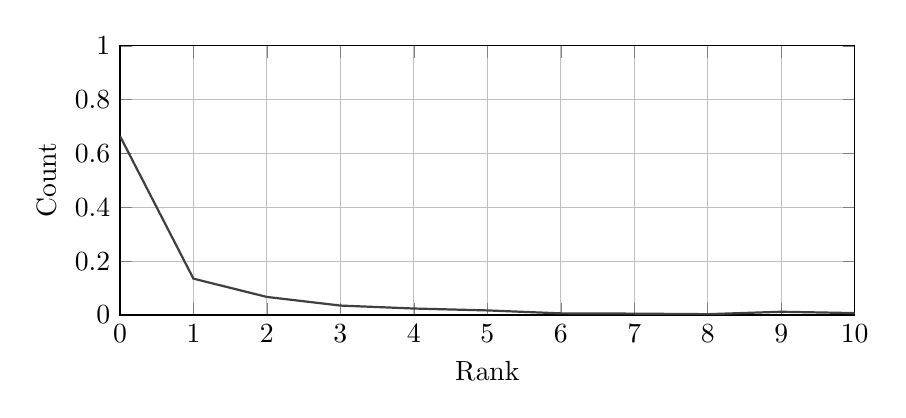
\begin{tikzpicture}[xscale=1,yscale=1]
\begin{axis}[xmin=0,xmax=10,ymin=0.0,ymax=1.00,no markers,grid=both,xlabel=Rank,ylabel=Count,width=0.9\textwidth,height=5cm]
\addplot[color=darkgray,thick] coordinates {(0, 0.665) (1, 0.135) (2, 0.067) (3, 0.035) (4, 0.024) (5, 0.017) (6, 0.006) (7, 0.005) (8, 0.003) (9, 0.012) (10, 0.007) (11, 0.006) (12, 0.003) (13, 0.004) (14, 0.002) (15, 0.0) (16, 0.002) (17, 0.002) (18, 0.0) (19, 0.0) (20, 0.0) (21, 0.001) (22, 0.002) (23, 0.0) (24, 0.0) (25, 0.0) (26, 0.0) (27, 0.0) (28, 0.0) (29, 0.0) (30, 0.0) (31, 0.0) (32, 0.0) (33, 0.0) (34, 0.001) (35, 0.0) (36, 0.0) (37, 0.0) (38, 0.0) (39, 0.0) (40, 0.0) (41, 0.0) (42, 0.0) (43, 0.0) (44, 0.0) (45, 0.0) (46, 0.0) (47, 0.0) (48, 0.0) (49, 0.0) (50, 0.001)};
\end{axis}
\end{tikzpicture}
\caption{Distribution of right key component ranks for 1000 experiments on $n=25$, $t=2.3$, $d=1$, $\mathrm{p}_{success}=0.99$.}
\label{fig:ranks}
\end{figure}

\anonymous{Our implementation will be made available soon.}{Our implementation is available at \url{http://bitbucket.org/malb/bkw-lwe}.}


}

\section{Applications}
\label{sec:parameters}
In this section we apply Theorem~\ref{theorem:complexity1} to various sets of parameters suggested in the literature. In order to compute concrete costs we rely on numerical approximations in various places such as the computation of $p_j$. We used $2n-4n$ bits of precision for all computations, increasing this precision further did not appear to change our results. The solving step for $m$ of Lemma~\ref{lem:m} is accomplished by a simple search implemented in Sage \cite{sagemath}. As a subroutine of this search we rely on numerical integration which we performed using the mpmath library \cite{mpmath} as shipped with Sage. The Sage script used to derive all values in this section is available at \cite{albrecht:bitbucket2012}.

In all cases below we always set $\PrS = 0.99$ and $a := \lceil t\cdot \log_2 n\rfloor$ where $t$ is a small constant, which is consistent with the complexity of the BKW algorithm $q^{\bigO{n/\log_2(n)}} = 2^{\bigO{n}}$ if $q \in \poly$.

\subsection{Regev's Original Parameters}\label{sec:parameters:regev}
In \cite{regev:acm09} Regev proposes a simple public-key encryption scheme with the suggested parameters $q \approx n^2$ and $\alpha = 1/(\sqrt{n} \cdot \log_2^2 n\sqrt{2\pi})$. We consider the parameters in the range $n=32,\dots,256$. In our experiments $t=3.0$ produced the best results, i.e., higher values of $t$ resulted in $m$ growing too fast. Plugging these values into the formulas of Theorem~\ref{theorem:complexity1} we get an overall complexity of 
\begin{comment}
sage: n, m = var('n,m')
sage: assume(n>0)
sage: assume(m>0)
sage: q = n^2
sage: t, d, r = 3, 2, 2
sage: a = t*log(n)
sage: b = n/a
sage: repeat = n/d
sage: corrector = (q**d)/(q**d - 1)
sage: stage1a = (q**b-1)/2.0 * ( a*(a-1)/2.0 * (n+1) - b*a*(a-1)/4.0 - b/6.0 * ( (a-1)**3 + 3/2.0*(a-1)**2 + 1/2.0*(a-1) ) )
sage: stage1b = corrector * (repeat + 1)/2.0 * m * (a/2.0 * (n + 2))
sage: stage1  = stage1a + stage1b
sage: stage2  = repeat * m * q**d
sage: stage3  = (repeat + 1) * d * a * q**b/2.0
sage: nops = stage1 + stage2 + stage3
sage: nops = nops.simplify_full()
sage: num = nops.numerator()
sage: den = nops.denominator()
sage: ops = num.operands()
sage: f = sum(op for op in ops if op >= 0)/den # we throw away things that only make it smaller
sage: f.simplify_full()
\end{comment}
\begin{eqnarray*}
\frac{mn^9 + \frac{1}{6} \, 2^{\frac{2}{3}n} n^5  + {\left[{\left(3\, n + \frac{9}{2}\right)} \cdot \left(2^{\frac{2}{3}n}n^4 + 1\right)\right]} \log_2\left(n\right)^{2} + \frac{1}{6} \, n}{2 \, {\left(n^4 -1\right)}}\\
\end{eqnarray*}
operations in $\Zq$ after simplification.
If $m <2^{(\frac{2}{2.6}n)})$ then this expression is dominated by
$$\frac{\frac{1}{6} n^5 +  {\left(3 \, n^5 + \frac{9}{2}n^4\right)} \cdot \log_2\left(n\right)^2}{2 \, (n^4 - 1)} 2^{\frac{2}{3}n}\in 2^{\frac{2}{3}n + \bigO{\log n}}.$$
However, since we compute $m$ numerically, we have to rely concrete values for various $n$ to verify that with these settings indeed $m$ does not grow too fast. Table~\ref{tab:concrete_regev} lists the estimated number of calls to $\Ldis$ (``$\log_2 \#\Ldis $''), the estimated number of required ring (``$\log_2 \#\Zq $'') and bit (``$\log_2 \#\mathbb{Z}_2 $'')  operations, the costs in terms of ring operations for each of the three stages sampling, hypothesis testing and back substitution.

\begin{table}[!htb]
\begin{center}
\begin{tabular}{|r|r|r|r|r|r|r|r|r|r|} 
\hline
$n$ & $\log_2 m $ & \multicolumn{4}{|c|}{$\log_2 \#\Zq $ in} & $\log_2 \#\mathbb{Z}_2 $ & $\log_2 \#\Ldis $\\
\hline
    &                                & sample & hypo. & subs. & total & & \\
\hline
 32 &  19.93 &  32.76 &  34.94 &  29.31 &  35.25 &  38.57 &  25.64\\
 48 &  28.90 &  43.70 &  45.66 &  40.69 &  46.02 &  49.50 &  35.81\\
 64 &  34.22 &  54.36 &  52.22 &  51.86 &  54.85 &  58.43 &  45.87\\
 80 &  42.19 &  65.50 &  61.16 &  62.94 &  65.78 &  69.44 &  56.60\\
 96 &  49.83 &  76.52 &  69.58 &  73.91 &  76.75 &  80.47 &  67.31\\
112 &  58.79 &  87.51 &  79.22 &  84.84 &  87.72 &  91.49 &  78.02\\
128 &  67.44 &  98.46 &  88.44 &  95.75 &  98.67 & 102.48 &  88.74\\
144 &  76.40 & 109.35 &  97.91 & 106.61 & 109.56 & 113.40 &  99.43\\
160 &  86.37 & 120.23 & 108.34 & 117.46 & 120.43 & 124.30 & 110.12\\
176 &  97.34 & 131.09 & 119.71 & 128.29 & 131.28 & 135.18 & 120.82\\
192 & 106.30 & 141.93 & 129.06 & 139.10 & 142.12 & 146.04 & 131.51\\
208 & 117.27 & 152.76 & 140.37 & 149.91 & 152.95 & 156.89 & 142.20\\
224 & 128.56 & 163.57 & 151.98 & 160.70 & 163.76 & 167.72 & 152.88\\
240 & 139.52 & 174.37 & 163.24 & 171.48 & 174.56 & 178.54 & 163.57\\
256 & 150.49 & 185.17 & 174.49 & 182.26 & 185.35 & 189.35 & 174.25\\
\hline
\end{tabular}
\end{center}
\caption{Cost of solving Search-LWE for parameters suggested in \cite{regev:acm09} with $d=1,t=3,\PrS=0.99$ with BKW.}
\label{tab:concrete_regev}
\end{table}

\subsection{Lindner and Peikert's Parameters}
\label{sec:parameters:pqc}

In \cite{LindnerP10}, Lindner and Peikert propose new attacks and parameters for LWE. Table~\ref{tab:concrete_lp} lists concrete costs of the BKW algorithm for solving LWE under the parameter choices from \cite{LindnerP10} as interpreted in \cite{albrecht-fitzpatrick-cabracas-goepfert-schneider:bitbucket2013}. In our computations $t=2.7$ produced the best results, i.e., higher values of $t$ resulted in $m$ growing too fast.

\begin{table}[!htb]
\begin{center}
\begin{tabular}{|r|r|r|r|r|r|r|r|r|r|} 
\hline
$n$ & $\log_2 m $ & \multicolumn{4}{|c|}{$\log_2 \#\Zq $ in} & $\log_2 \#\mathbb{Z}_2 $ & $\log_2 \#\Ldis $\\
\hline
    &                                & sample & hypo. & subs. & total & & \\
\hline
 32 &   7.64 &  35.91 &  33.65 &  33.92 &  36.46 &  39.78 &  28.84\\
 48 &   9.97 &  45.75 &  36.56 &  43.58 &  46.04 &  49.52 &  37.94\\
 64 &  15.61 &  54.82 &  42.62 &  52.53 &  55.09 &  58.67 &  46.49\\
 80 &  22.25 &  63.39 &  49.58 &  61.02 &  63.65 &  67.31 &  54.66\\
 96 &  30.90 &  71.62 &  58.49 &  69.18 &  71.86 &  75.58 &  62.57\\
112 &  40.86 &  79.57 &  68.68 &  77.08 &  79.81 &  83.58 &  70.25\\
128 &  54.15 &  87.32 &  82.16 &  84.78 &  87.58 &  91.39 &  77.76\\
144 &  37.54 & 102.31 &  67.71 &  99.73 & 102.53 & 106.37 &  92.54\\
160 &  46.51 & 110.38 &  76.83 & 107.77 & 110.60 & 114.47 & 100.43\\
176 &  56.47 & 118.31 &  86.93 & 115.68 & 118.53 & 122.43 & 108.20\\
192 &  70.76 & 126.13 & 101.35 & 123.47 & 126.34 & 130.26 & 115.87\\
208 &  80.73 & 133.84 & 111.43 & 131.15 & 134.05 & 137.99 & 123.44\\
224 &  94.34 & 141.45 & 125.15 & 138.74 & 141.66 & 145.62 & 130.92\\
240 & 109.62 & 148.98 & 140.53 & 146.25 & 149.18 & 153.16 & 138.33\\
256 & 126.23 & 156.42 & 157.24 & 153.68 & 157.96 & 161.96 & 145.67\\
\hline                                                                                                 
\end{tabular}
\end{center}
\caption{Cost of solving Search-LWE for parameters suggested in \cite{LindnerP10} with $d=1,t=2.7, \PrS=0.99$ with BKW.}
\label{tab:concrete_lp}
\end{table}

\subsection{Albrecht et al.'s Polly-Cracker}
\label{sec:parameters:polly}

In \cite{albrecht-farshim-faugere-perret:asiacrypt2011} a somewhat homomorphic encryption scheme is proposed based on the hardness of computing Gröbner bases with noise. Using linearisation the equation systems considered in \cite{albrecht-farshim-faugere-perret:asiacrypt2011} may be considered as LWE instances. Table~\ref{tab:concrete_polly} lists concrete costs for recovering the secret Gröbner basis using this strategy for selected parameters suggested in \cite{albrecht-farshim-faugere-perret:asiacrypt2011}. In Table~\ref{tab:concrete_polly} ``$\lambda$'' is the targeted bit-security level and $n$ the number of variables in the linearised system. We note that we did not exploit the structure of the secret for Table~\ref{tab:concrete_polly}.


\begin{table}[!htb]
\begin{center}
\begin{tabular}{|r|r|r|r||r||r|r|r|r|r|r|r|r|r|} 
\hline
$\lambda $ & $n$ & $q$ & $\alpha$ & $t$ & $\log_2 m $ & \multicolumn{4}{|c|}{$\log_2 \#\Zq $ in} & $\log_2 \#\mathbb{Z}_2 $ & $\log_2 \#\Ldis $\\
\hline
& & &    &              &                 &  sample & hypo. & subs. & total & &\\
\hline
 80 &  136 &   1999 & 0.005582542\dots & 2.2 &  93.58 & 109.40 & 121.59 & 105.71 & 121.59 & 125.04 & 100.23\\ 
    &  231 &  92893 & 0.000139563\dots & 3.4 & 127.23 & 157.47 & 167.09 & 154.40 & 167.09 & 171.13 & 146.54\\
\hline                                                                                                    
128 & 153 &  12227 & 0.002797408\dots & 2.4 &  84.05 & 132.07 & 117.45 & 129.66 & 132.32 & 136.08 & 122.39\\
    & 253 & 594397 & 0.000034967\dots & 3.8 & 100.66 & 175.15 & 146.00 & 171.88 & 175.29 & 179.55 & 163.89\\
\hline
\end{tabular}
\end{center}
\caption{Cost of finding $G \approx \svec$ for parameters suggested in \cite{albrecht-farshim-faugere-perret:asiacrypt2011} with $d=2, \PrS=0.99$.}
\label{tab:concrete_polly}
\end{table}



\section{Conclusion \& Future Work}

We investigated applying modulus switching to exploit the presence of a small secret in LWE instances and demonstrated that it can make a significant impact on the complexity of solving such instances. We also adapted the BKW algorithm to perform modulus-switching `on-the-fly', showing that this approach is superior to performing `one-shot' modulus reduction on LWE samples prior to solving. Our first variant improves the target modulus by a factor of $\sqrt{\log_2 n}$ in typical scenarios; our second variant mainly improves the memory requirements of the algorithm, one of the key limiting aspects of the BKW algorithm. Our algorithms, however, rely on various assumptions which, though appearing sound, are unproven. Our estimates should thus be considered heuristic, as are performance estimates for all currently-known algorithms for solving LWE. Verifying these assumptions is hence a promising direction for future research. Furthermore, one of the main remaining obstacles for applying the BKW algorithm to cryptographic constructions based on LWE is that it requires an unbounded number of samples to proceed. Lifting this requirement, if only heuristically, is hence a pressing research question.

\section*{Acknowledgement}
We thank Steven Galbraith for helpful comments on an earlier draft of this work. We also thank anonymous referees for detailed comments which greatly improved this work. Jean-Charles Faugère, and Ludovic Perret  have been partially supported supported by the Computer Algebra and Cryptography (CAC) project (ANR-09-JCJCJ-0064-01) and the HPAC grant (ANR ANR-11-BS02-013) of the French National Research Agency. 

\bibliographystyle{plain}
\bibliography{bkw-small-secret}

\end{document}
